%%%%%%%%%%%%%%%%%%%%%%%%%%%%%%%%%%%%%%%%%%%%%%%%%%%%%%%%%%%%%%%%%%%%%%%%%%%%%
%%%  Updated by Lenore Cowen and Mengfei Cao, version 4.0, December 2015
%%%%
%%%% We believe this template now meets the style requirements for a PHD 
%%% dissertation at Tufts University, but you still need to check this with
%%% the Tufts University graduate handbook, currently located at 
%%% http://asegrad.tufts.edu/sites/default/files/GraduateStudentHandbook.pdf
%%% starting at page 25 to make sure your final document is in compliance.
%%%%% 
%%% Updated by Anoop Kumar, version 3.0, February 2010
%%% 
%%% File: utthesis2.doc, version 2.0jab, February 2002
%%%
%%% Based on: utthesis.doc, version 2.0, January 1995
%%% =============================================
%%% Copyright (c) 1995 by Dinesh Das.  All rights reserved.
%%% This file is free and can be modified or distributed as long as
%%% you meet the following conditions:
%%%
%%% (1) This copyright notice is kept intact on all modified copies.
%%% (2) If you modify this file, you MUST NOT use the original file name.
%%%
%%% This file contains a template that can be used with the package
%%% utthesis.sty and LaTeX2e to produce a thesis that meets the requirements
%%% of the Graduate School of The University of Texas at Austin.
%%%
%%% All of the commands defined by utthesis.sty have default values (see
%%% the file utthesis.sty for these values).  Thus, theoretically, you
%%% don't need to define values for any of them; you can run this file
%%% through LaTeX2e and produce an acceptable thesis, without any text.
%%% However, you probably want to set at least some of the macros (like
%%% \thesisauthor).  In that case, replace "..." with appropriate values,
%%% and uncomment the line (by removing the leading %'s).
%%%
%%%%%%%%%%%%%%%%%%%%%%%%%%%%%%%%%%%%%%%%%%%%%%%%%%%%%%%%%%%%%%%%%%%%%%%%%%%%%

\documentclass[11pt,pdflatex]{report}         %% LaTeX2e document.
\usepackage {thesis}              %% Preamble.
\usepackage {url}
\usepackage {graphicx}
\usepackage {subfigure}
\usepackage {fancyvrb}
\usepackage {algorithm}
\usepackage {algorithmic}
\usepackage[usenames]{color}
\usepackage{listings}
\usepackage{amsmath}
\usepackage{amssymb}
\usepackage{multirow}
\usepackage{ctable}
\usepackage{tabulary} 

%\usepackage{fullpage, setspace}

% \mastersthesis                     %% Uncomment one of these; if you don't
%\phdthesis                         %% use either, the default is \phdthesis.

%\thesisdraft                       %% Uncomment this if you want a draft
                                     %% version; this will print a timestamp
                                     %% on each page of your thesis.

% \leftchapter                       %% Uncomment one of these if you want
% \centerchapter                     %% left-justified, centered or
% \rightchapter                      %% right-justified chapter headings.
                                     %% Chapter headings includes the
                                     %% Contents, Acknowledgments, Lists
                                     %% of Tables and Figures and the Vita.
                                     %% The default is \centerchapter.

% \singlespace                       %% Uncomment one of these if you want
%\oneandhalfspace                   %% single-spacing, space-and-a-half
%\doublespace                       %% or double-spacing; the default is
                                     %% \oneandhalfspace, which is the
                                     %% minimum spacing accepted by the
                                     %% Graduate School.

\renewcommand{\thesisauthor}{Anuththari Gamage}    %% Your name.

\renewcommand{\thesismonth}{May}   %% Your month of graduation.

\renewcommand{\thesisyear}{2018}      %% Your year of graduation.

% \renewcommand{\thesistitle}{System Design, Testing, Deployment, and
% Management in a Component-based and Autonomic Way\\
% Offloading System Management Tasks to Distributed Appliances}

%\renewcommand{\thesistitle}{Augmented Training  Methods for Hidden Markov Model%s for the Detection of Remote Protein Homologs}

\renewcommand{\thesistitle}{Tensor Methods for Multi-layer Graph Embedding}

                                     %% The title of your thesis; use
                                     %% mixed-case.

\renewcommand{\thesisauthorpreviousdegrees}{}
                                     %% Your previous degrees, abbreviated;
                                     %% separate multiple degrees by commas.

\renewcommand{\thesissupervisor}{Prof. Shuchin Aeron}
                                     %% Your thesis supervisor; use mixed-case
                                     %% and don't use any titles or degrees.

% \renewcommand{\thesiscosupervisor}{}
                                     %% Your PhD. thesis co-supervisor; if any.
                                     %% Use mixed case and don't use any titles
                                     %% or degrees. Uncomment if you
                                     %% have a co-supervisor.
                                     %% (Ignored for Master's)

\renewcommand{\thesiscommitteemembera}{Prof. Misha Kilmer}
\renewcommand{\thesiscommitteememberb}{Prof. Xiaozhe Hu}
%\renewcommand{\thesiscommitteememberc}{Prof. Other Tufts}
%\renewcommand{\thesiscommitteememberd}{Prof. Mo Willems}
% \renewcommand{\thesiscommitteemembere}{}
% \renewcommand{\thesiscommitteememberf}{}
% \renewcommand{\thesiscommitteememberg}{}
% \renewcommand{\thesiscommitteememberh}{}
% \renewcommand{\thesiscommitteememberi}{}
                                     %% Define your other committee members here;
                                     %% use mixed case and don't use any titles
                                     %% or degrees.  Uncomment as many
                                     %% as neccessary. (Ignored for Master's)

\renewcommand{\thesisauthoraddress}{
Tufts University\\
161 College Ave.
Medford, MA 02155}
                                     %% Your permanent address; use "\\" for
                                     %% linebreaks.

\renewcommand{\thesisdedication}{{\em To everyone who helped me get to grad school, helped me in grad school, or simply managed to put up with me while I was in graduate school. And to the people who finally let me leave.}}
                                     %% Your dedication, if you have one; use
                                     %% "\\" for linebreaks.

\newtheorem{theorem}{Theorem}[section]
\newtheorem{lemma}[theorem]{Lemma}
\newtheorem{proposition}[theorem]{Proposition}
\newtheorem{corollary}[theorem]{Corollary}

\newenvironment{proof}[1][Proof]{\begin{trivlist}
\item[\hskip \labelsep {\bfseries #1}]}{\end{trivlist}}
\newenvironment{definition}[1][Definition]{\begin{trivlist}
\item[\hskip \labelsep {\bfseries #1}]}{\end{trivlist}}
\newenvironment{example}[1][Example]{\begin{trivlist}
\item[\hskip \labelsep {\bfseries #1}]}{\end{trivlist}}
\newenvironment{remark}[1][Remark]{\begin{trivlist}
\item[\hskip \labelsep {\bfseries #1}]}{\end{trivlist}}

\newcommand{\qed}{\nobreak \ifvmode \relax \else
      \ifdim\lastskip<1.5em \hskip-\lastskip
      \hskip1.5em plus0em minus0.5em \fi \nobreak
      \vrule height0.75em width0.5em depth0.25em\fi}
\newcommand{\toEdit}[1]{\textcolor{red}{{\em #1}}}
\newcommand{\comment}[1]{\textcolor{blue}{\em{\sc{#1}}}}

%%%%%%%%%%%%%%%%%%%%%%%%%%%%%%%%%%%%%%%%%%%%%%%%%%%%%%%%%%%%%%%%%%%%%%%%%%%%%
%%%
%%% The following commands are all optional, but useful if your requirements
%%% are different from the default values in utthesis.sty.  To use them,
%%% simply uncomment (remove the leading %) the line(s).

% \renewcommand{\thesiscommitteesize}{5}
                                     %% Uncomment this only if your thesis
                                     %% committee does NOT have 5 members
                                     %% for \phdthesis or 2 for \mastersthesis.
                                     %% Replace the "..." with the correct
                                     %% number of members.

 \renewcommand{\thesisdegree}{Bachelor of Science}  %% Uncomment this only if your thesis
                                     %% degree is NOT "DOCTOR OF PHILOSOPHY"
                                     %% for \phdthesis or "MASTER OF ARTS"
                                     %% for \mastersthesis.  Provide the
                                     %% correct FULL OFFICIAL name of
                                     %% the degree.

 \renewcommand{\thesisdegreeabbreviation}{B.S.}
                                     %% Use this if you also use the above
                                     %% command; provide the OFFICIAL
                                     %% abbreviation of your thesis degree.

 \renewcommand{\thesistype}{Senior Honors Thesis}    %% Use this ONLY if your thesis type
                                     %% is NOT "Dissertation" for \phdthesis
                                     %% or "Thesis" for \mastersthesis.
                                     %% Provide the OFFICIAL type of the
                                     %% thesis; use mixed-case.

% \renewcommand{\thesistypist}{...}  %% Use this to specify the name of
                                     %% the thesis typist if it is anything
                                     %% other than "the author".

%%%
%%%%%%%%%%%%%%%%%%%%%%%%%%%%%%%%%%%%%%%%%%%%%%%%%%%%%%%%%%%%%%%%%%%%%%%%%%%%%

\begin{document}

%\thesiscopyrightpage                 %% Generate the copyright page.

%\thesiscertificationpage             %% Generate the PhD. certification page.

\thesistitlepage                     %% Generate the title page.

%\thesissignaturepage                %% Generate the Master's signature page.

%\thesisdedicationpage                %% Generate the dedication page.


\begin{thesisacknowledgments}        %% Use this to write your acknowledgments; it can be anything allowed in LaTeX2e par-mode.

The work described in this dissertation is the result of many people's helpful advice, useful suggestion and enthusiastic contribution. 

Thank everyone who has helped in the work

%% Uncomment out if needed: 
%% Portions of this work have been previous published as PAPER1 PAPER2 PAPER3.
%% I thank my co-authors for their permission to include our joint published
%%% work in this thesis. 

\end{thesisacknowledgments}
  %%% Goto acknowledgement.tex for content

\begin{thesisabstract}
 

 The abstract goes here.
\nopagebreak
\end{thesisabstract}   %%% Goto abstract.tex for content


\tableofcontents                   %% Generate table of contents.
\listoftables                      %% Uncomment this to generate list
                                   %% of tables.
\listoffigures                     %% Uncomment this to generate list
                                   %% of figures.
\chapter{Introduction}

\label{chapter:introduction}

This is the introductory chapter. I am going to tell you all the background and definitions you need to understand the material in Chapter~\ref{chapter:chapter2} and Chapter~\ref{chapter:chapter3}).


\section{First Background Section }



\subsection{Something About this}

Here is some text. And it describes some evidence that is found in
Figure~\ref{elephantfig}.


\begin{figure}[htb!]
\begin{center}
  \fbox{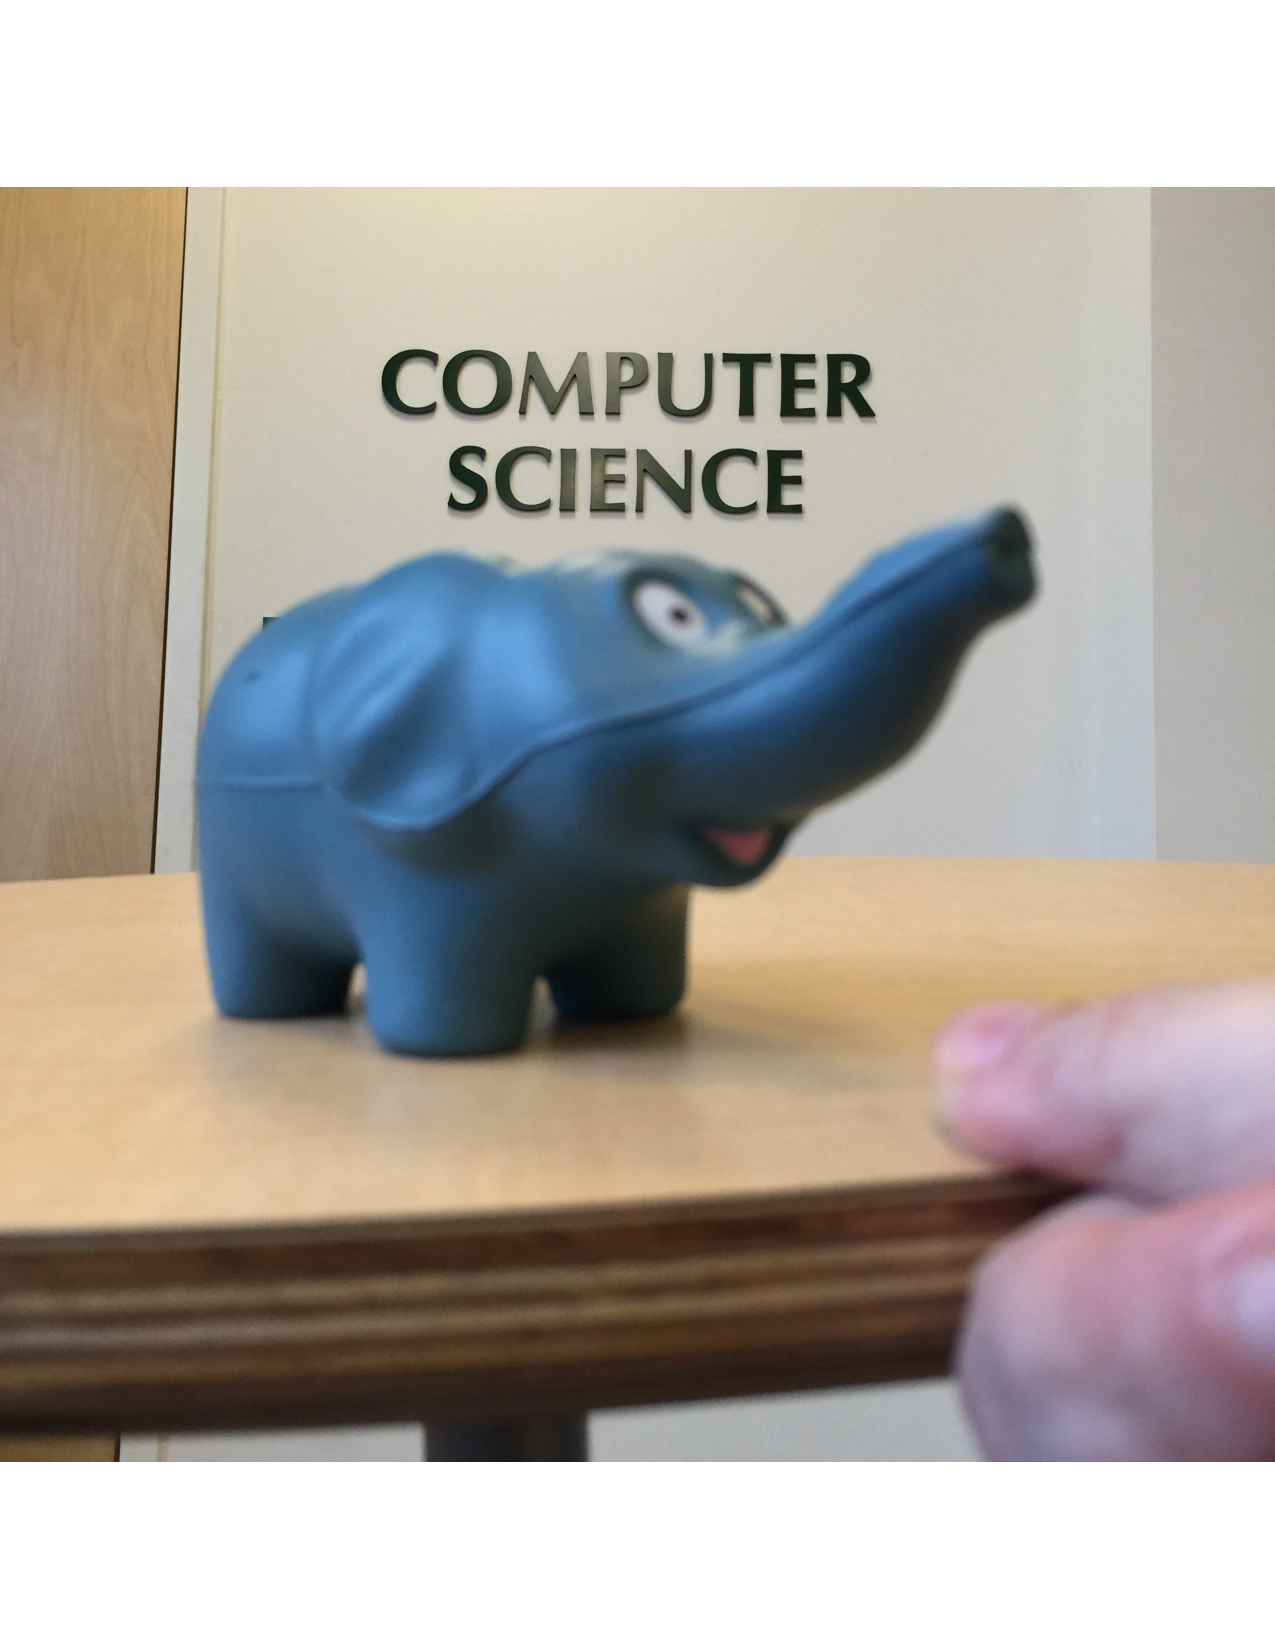
\includegraphics[height=4.5in]{cs-focus.pdf}}
   \caption{The footprints in the margarine}
   \label{elephantfig}
 \end{center}
\end{figure}


\section{Outline of This Work}

Following is the  outline  of individual chapters in this thesis.

In Chapter 2, we show the trunk.

In Chapter 3, we discuss the search space. 

Finally in Chapter 4, we discuss the results and summarize the key
findings of this thesis followed by possible directions of future
work.
             
\chapter{Review of Related Literature} 

\label{chapter:chapter2}

\section{Multilayer Graph Embedding}
\subsection{Tensor Factorization methods}

\subsection{Spectral Methods}

\subsection{Other methods}

\section{Pros and Cons of these approaches}





%\section{Some background } 


%
%In order to study the trunk of the elephant, my best beloved, we have so many stories to tell you~\cite{kipling2010just}. 
%
%Assume that the trunk consists of $N$ different segments. On the other hand, it is always important to cite the crucial work in the field~\cite{willems2007there}.
%
%%%%%%%%%%%%%%%%%%%%%%%%%%%%%%%%%%%%%%%%
%
%\section{Results} 
%
%
%\subsection{Elephant color scales}
%
%\begin{table}[htb!]
%   \begin{center}
%      \begin{tabular}{|l|l|l|l|l|l|l|} \hline
%      {\bf Class} & {\bf African} & {\bf Asian}  & {\bf Martian}  & {\bf Cartoon}  & {\bf Plush} & {\bf Plastic} \\\hline
%      {\bf Body} &  0.57  & 0.21 & 0.31 & 0.40 & 0.46 & 0.30 \\\hline
%      {\bf Tusk} & 0.85 & 0.87 & 0.87 & 0.91 & 0.93 & 0.93 \\\hline
%      {\bf Trunk} & 1.00  & 0.94 & 0.97 & 0.97 & 0.97 & 1.00 \\\hline
%      {\bf Ear} & 0.73  & 0.73 & 0.64 & 0.73 & 1.00 & 0.82 \\\hline
%      {\bf Tail} & 0.67 & 1.00 & 1.00 & 1.00 & 1.00 & 1.00 \\\hline
%      \end{tabular}
%   \end{center}
%   \caption{Careful measurements in cross-validation. Note that it is easier to get a plush or plastic elephant to stay still and be measured, so those measurements are deemed more reliable. Cartoon elephants require special cleverness and a deep knowledge of cartoon physics to measure with motion capture technology.}
%   \label{gpcr_coverage}
%\end{table}
%
%
%%%%%%%%%%%%%%%%%%%%%%%%%%%%%%%%%%
%
   
\chapter{Methodology} 

\label{chapter:chapter3}

%\section{Hunting for the elephant} 
%
%Jim Huggins has posted some interesting information about how to hunt
%elephants but all attempts to hunt down the citation have failed, so
%we cannot include a description in this thesis.
%
%
%%%%%%%%%%%%%%%%%%%%%%%%%%%%%%%%%%%%%%%%
%
%\section{Results} 
%
%(None) 
%%%%%%%%%%%%%%%%%%%%%%%%%%%%%%%%%%

         
\chapter{Evaluation and Findings}  
\label{chapter:chapter4}

They claim an elephant never forgets, but that is probably wrong. They
say the Internet never forgets, but that is also probably wrong. We
forget things all the time. In the future, I hope that future students
who pass on this template each leave at least one new elephant joke,
latex use example, or elephant citation to continue the field of Jumbo
Studies which is still in its infancy.


                
                  

%================================ END of chapters =============================

\addcontentsline {toc}{chapter}{Bibliography}
                                     %% Force Bibliography to appear in contents

%\begin{thebibliography}{..}          %% Start your bibliography here; you can
%\bibitem{...} ...                    %% also use the \bibliography command
%\end{thebibliography}                %% to generate your bibliography.

\bibliographystyle{alpha}
\bibliography{thesis}

%\begin{thesisauthorvita}             %% Write your vita here; it can be
%...                                  %% anything in LaTeX2e par-mode.
%\end{thesisauthorvita}               %%

\end{document}                       %% Done.
